
\documentclass[a4paper,12pt]{report}
\usepackage{graphicx}
\usepackage{booktabs}
\usepackage{amsmath}
\usepackage{listings}
\usepackage[stable]{footmisc}
\title{MATLAB Model and Data Structures}
\begin{document}
	

\maketitle
\tableofcontents


	
\chapter{Calling Sequence}	

		\lstinputlisting{call.m}
	
	
\chapter{Model structure (idpoly)}
	
	
	\section{Model structure output \footnote{\label{dj}This option is also available in GUI (called using 'ident')}}
	

	\begin{enumerate}
		\item Type of model : discrete-time\footref{dj}
		\item Type of estimation method 
		\item Equation showing relation between polynomials  
		\item Model representation (A,B,C polynomials in increasing power of $z^{-1}$)
			
		\item Sample time
		
		\item Parameterization : Polynomial orders, Number of free parameters
		\item Hint for functions that can be used for extra information like uncertainties in polynomial values and their covariance 
		\item Information about whether the model is constructed with fixed parameters or estimated from data
		\item Information about the data used to estimate the model
		\item Fit percentage, Final Prediction Error(FPE), Mean Squared Error(MSE)
		\item Focus -  Error to be minimized ('prediction' or 'simulation')
	
			
			
			
			
			
			\begin{figure}[tbp]
				\centering
				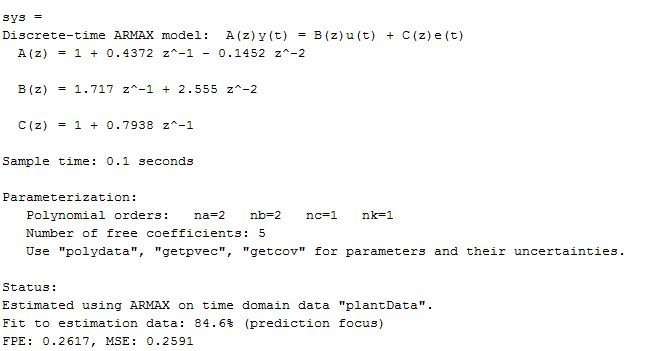
\includegraphics[width=0.8\textwidth]{modMat1.JPG}
				\caption{Model Output}
				\label{}
			\end{figure}
			
		\end{enumerate}	
			
		\section{Model structure attributes}	
			
		\begin{enumerate}	
			\item Polynomial coefficients vector
			
			\item Addition of integrators in noise channel \footref{dj}
			
			\item Variable('$z^{-1}$') used in polynomials
			
			\item Transport delays for each input/output pair using IODelay
		
			\item Following information about each polynomial :
		\begin{enumerate}
			
			\item Parameter values
			\item Upper and lower bounds on values
			\item Property of each coefficient - Tunable or not
			\item Scaling factor used to normalize the parameter value
			\item Unit and label for each parameter
		
		\end{enumerate}
		
		\item Value of variance of noise channel
		
		\item Detailed report with following information :  
		
		\begin{enumerate}
			\item Status : model is constructed or estimated
			\item Estimation method used 
			\item Handling of initial conditions during estimation, specified as one of the following values : 'zero', 'estimate', 'backcast', 'auto' \footref{dj}
			\item Values of Mean Squared Error(MSE), Final Prediction Error(FPE), Fit Percentage, Raw Akaike's Information Criterion(AIC), Small sample-size corrected (AICc), Normalized AIC(nAIC), Bayesian information criteria(BIC), Loss function
			\item Information about parameters (free parameters vector, covariance, and label) \footref{dj}
			\item Following options are available in OptionsUsed structure :
			
			\begin{enumerate}
				\item Initial condition
				\item Specifying whether to display the estimation progress ('off' or 'on') \footref{dj}
				\item Input and output offset
				\item Controlling whether parameter covariance data is generated \footref{dj}
				\item Regularized estimation of model parameters using a constant that determines the bias versus variance tradeoff \footref{dj}
				\item Following search methods available for iterative parameter estimation :
				\begin{enumerate}
					\item Subspace Gauss-Newton least squares search
					\item Adaptive subspace Gauss-Newton search
					\item Levenberg-Marquardt least squares search
					\item Steepest descent least squares search
					\item Non-linear least squares solver
					\item Constrained non-linear solvers
				\end{enumerate}
				
				\item Following search options are available :
				\begin{enumerate}
					\item Tolerance
					\item Maximum iterations
					\item Step tolerance, function tolerance
				\end{enumerate}
				
				\item Focus - Error to be minimized ('prediction' or 'simulation') \footref{dj} 
				\item Following options for weighting filter are available 
			\begin{enumerate}
				\item Passbands — Specify a row vector or matrix containing frequency values that define desired passbands
				\item SISO filter
			\end{enumerate}
				\item Controlling whether to enforce stability of estimated model (estimated model must be stable) \footref{dj}
				\item Following advanced options are available :
				\begin{enumerate}
					\item Error threshold to specify when to adjust the weight of large errors from quadratic to linear
					\item Max Size to specify maximum number of elements in a segment when input-output data is split into segments
					\item AutoInitThreshold to specify when to automatically estimate the initial condition
				\item	StabilityThreshold to specify thresholds for stability tests
					
	\end{enumerate}
\end{enumerate}
				
			\item Controlling random number generation at the start of estimation
			\item Information about data used for estimation - type of data, length, sample time, offset in input or output, input intersample behaviour 
			\item Following termination conditions for the iterative search used for prediction error minimization :
			\begin{enumerate}
				\item Reason
				\item Number of iterations performed
				\item Infinity norm of the gradient search vector when the search algorithm terminates
				\item Number of function call
				\item Norm of the gradient search vector in the last iteration
				\item Criterion improvement in the last iteration
				\item Algorithm used by 'lsqnonlin' or 'fmincon' search method
			\end{enumerate}
				
				
				
				
				
				
				
			\end{enumerate}
		
		
		
		
		
		
		
		
		
		
		
		
		
	
		\item Input Delay \footref{dj}
	\item Output Delay
	\item Sample time
	\item Time unit
	\item Name of input data vector (If not specified, default name 'u1')
	\item Input unit
	\item Input channel groups to assign input channels of MIMO systems into groups and refer to each group by name
	\item Name of output data vector (If not specified, default name 'y1')
	\item Output unit
	\item Output channel groups to assign output channels of MIMO systems into groups and refer to each group by name
			
	\item Notes in the form of string (An arbitrary field to store extra information)
	
	\item Any other user data/comments
	
	\item Any arbitrary name for model 
	\item Sampling grid for model arrays, specified as a data structure
		
		
		
	
		
		
			
	\end{enumerate}
			
			
			
		
		\begin{figure}[tbp]
			\centering
			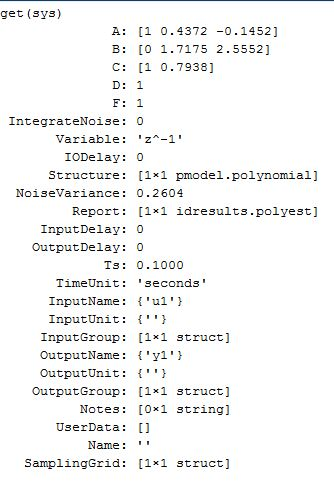
\includegraphics[width=0.8\textwidth]{modMat2.JPG}
			\caption{Model attributes}
			\label{}
		\end{figure}
	
		\begin{figure}[tbp]
		\centering
		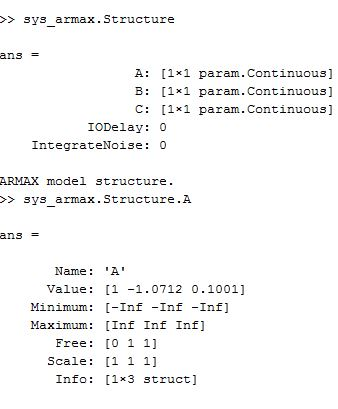
\includegraphics[width=0.8\textwidth]{StruMat.JPG}
		\caption{sys.Structure}
		\label{}
	\end{figure}
	
	
	
	\begin{figure}[tbp]
		\centering
		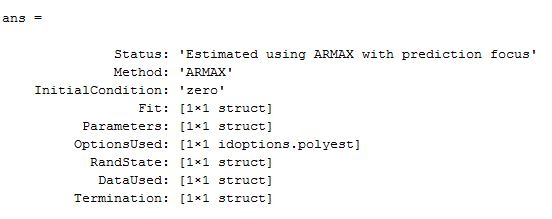
\includegraphics[width=0.8\textwidth]{repMat.JPG}
		\caption{sys.Report}
		\label{}
	\end{figure}
	
				
			\begin{figure}[tbp]
				\centering
				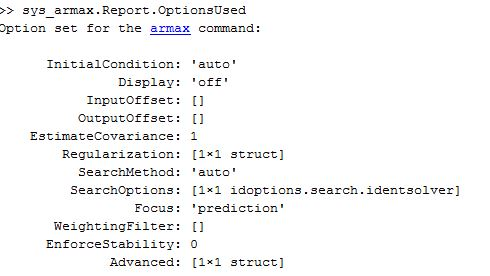
\includegraphics[width=0.8\textwidth]{OptMat.JPG}
				\caption{sys.Report.OptionsUsed}
				\label{}
			\end{figure}
			\chapter{Data structure (iddata)}
			\section{Data structure output}
		
			 
			\begin{enumerate}
				\item Domain of data : Time or frequency
				\item Number of samples
			\item Sample time
			\item Output vector name
			\item Output unit 
			\item Input vector name
		\item Input unit
			
		\end{enumerate}
	\section{Data structure attributes}
			
			
			
			\begin{enumerate}
			
			\item Domain of data : Time or frequency	
			\item Any arbitrary name for data 
				
			\item Output data vector stored in OutputData
			
			\item Output data vector stored in y
				
				\item Name of output vector which is displayed on iddata call (If not specified, default names, {'y1';'y2';...})
				
				 \item Output unit
				 	\item Input data vector stored in InputData
				 
				 \item Input data vector stored in u
				 
				 \item Name of input vector which is displayed on iddata call (If not specified, default names, {'u1';'u2';...})
				 
				 \item Input unit
			
				
				\item Period of input data 
			
			\item Inter sample behaviour of input : 'zoh', 'foh', or 'bl', depending on whether data is piecewise constant, piecewise linear, or band limited
				
			\item Sample time
				
			\item Starting time instant stored in Tstart
				
				\item Time instants stored in a vector
				
			\item Time unit
				
			\item Name of experiment (iddata can store data of multiple experiments)
				
		\item Notes in the form of string (An arbitrary field to store extra information)
				
			\item Any other user data/comments
			\end{enumerate}
			
			
			\begin{figure}[tbp]
				\centering
				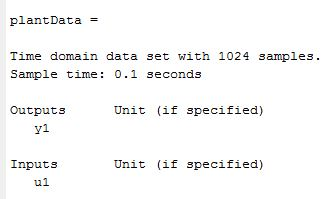
\includegraphics[width=0.8\textwidth]{datMat1.JPG}
				\caption{Data Output}
				\label{}
			\end{figure}
		
		\begin{figure}[tbp]
			\centering
			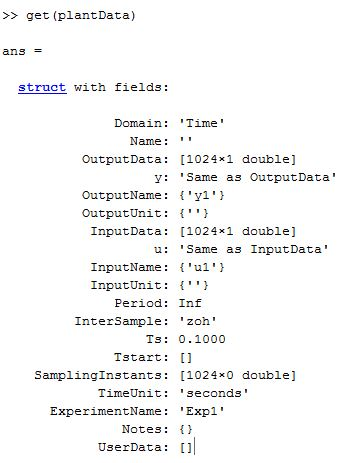
\includegraphics[width=0.8\textwidth]{datMat.JPG}
			\caption{Data attributes}
			\label{}
		\end{figure}
			
%\chapter{Data structure (iddata)}




\end{document}
